
\section{Results}

We collected 18 fecal and 23 oral microbiome samples from two identical twin human astronauts, one flight subject (TW, 9 stool, 6 saliva, 5 buccal) and one control who did not leave earth (HR, 9 stool, 7 saliva, 5 buccal), taken from 2014-2018. These were compared to 42 time-matched, environmental samples from the ISS that corresponded to the flight subject's mission duration. All samples were sequenced with 2x150bp read length to a mean depth of ~12-15M reads (12.01, 14.96, and 14.97M mean reads for ISS, fecal, and saliva, respectively), then aligned to the catalog of NCBI RefSeq complete microbial genomes, examined for single nucleotide polymorphisms (SNPs), and then run with strain analysis with the MetaSUB CAP pipeline and Aldex2 (see methods). 

\subsection{Taxonomic profiles show evidence of continual microbial exchange}

\begin{figure}
  \begin{center}
    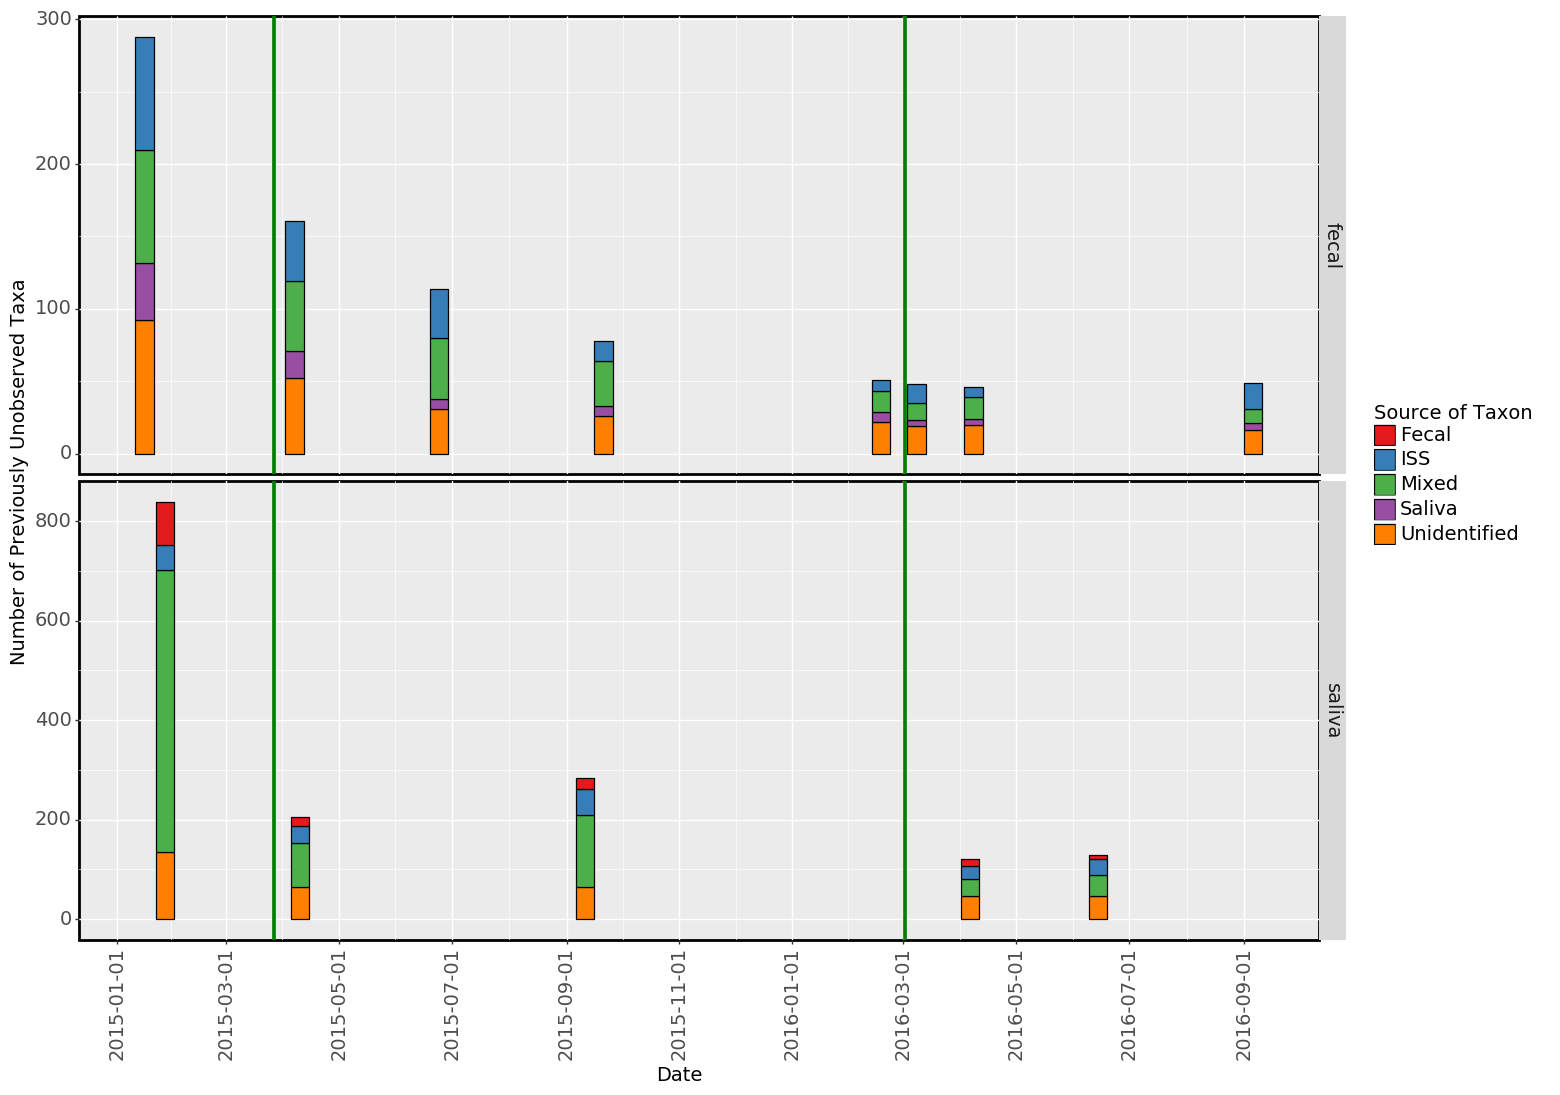
\includegraphics[width=0.99\textwidth]{figs/twins_taxa_sources.png}
%	\vspace{-20pt}
	\caption{\small{
	    This plot shows the number of taxa at each time point that were not observed at any previous timepoint for fecal and saliva samples from TW. The colors indicate the likely source of the new taxon if it was found previously in the saliva (for fecal samples, vice versa for saliva samples), the ISS, both (Mixed), or neither.
	}}
    \label{fig:taxasource}
  \end{center}
%  \vspace{-20pt}
 % \vspace{1pt}
\end{figure}

\begin{figure}
  \begin{center}
    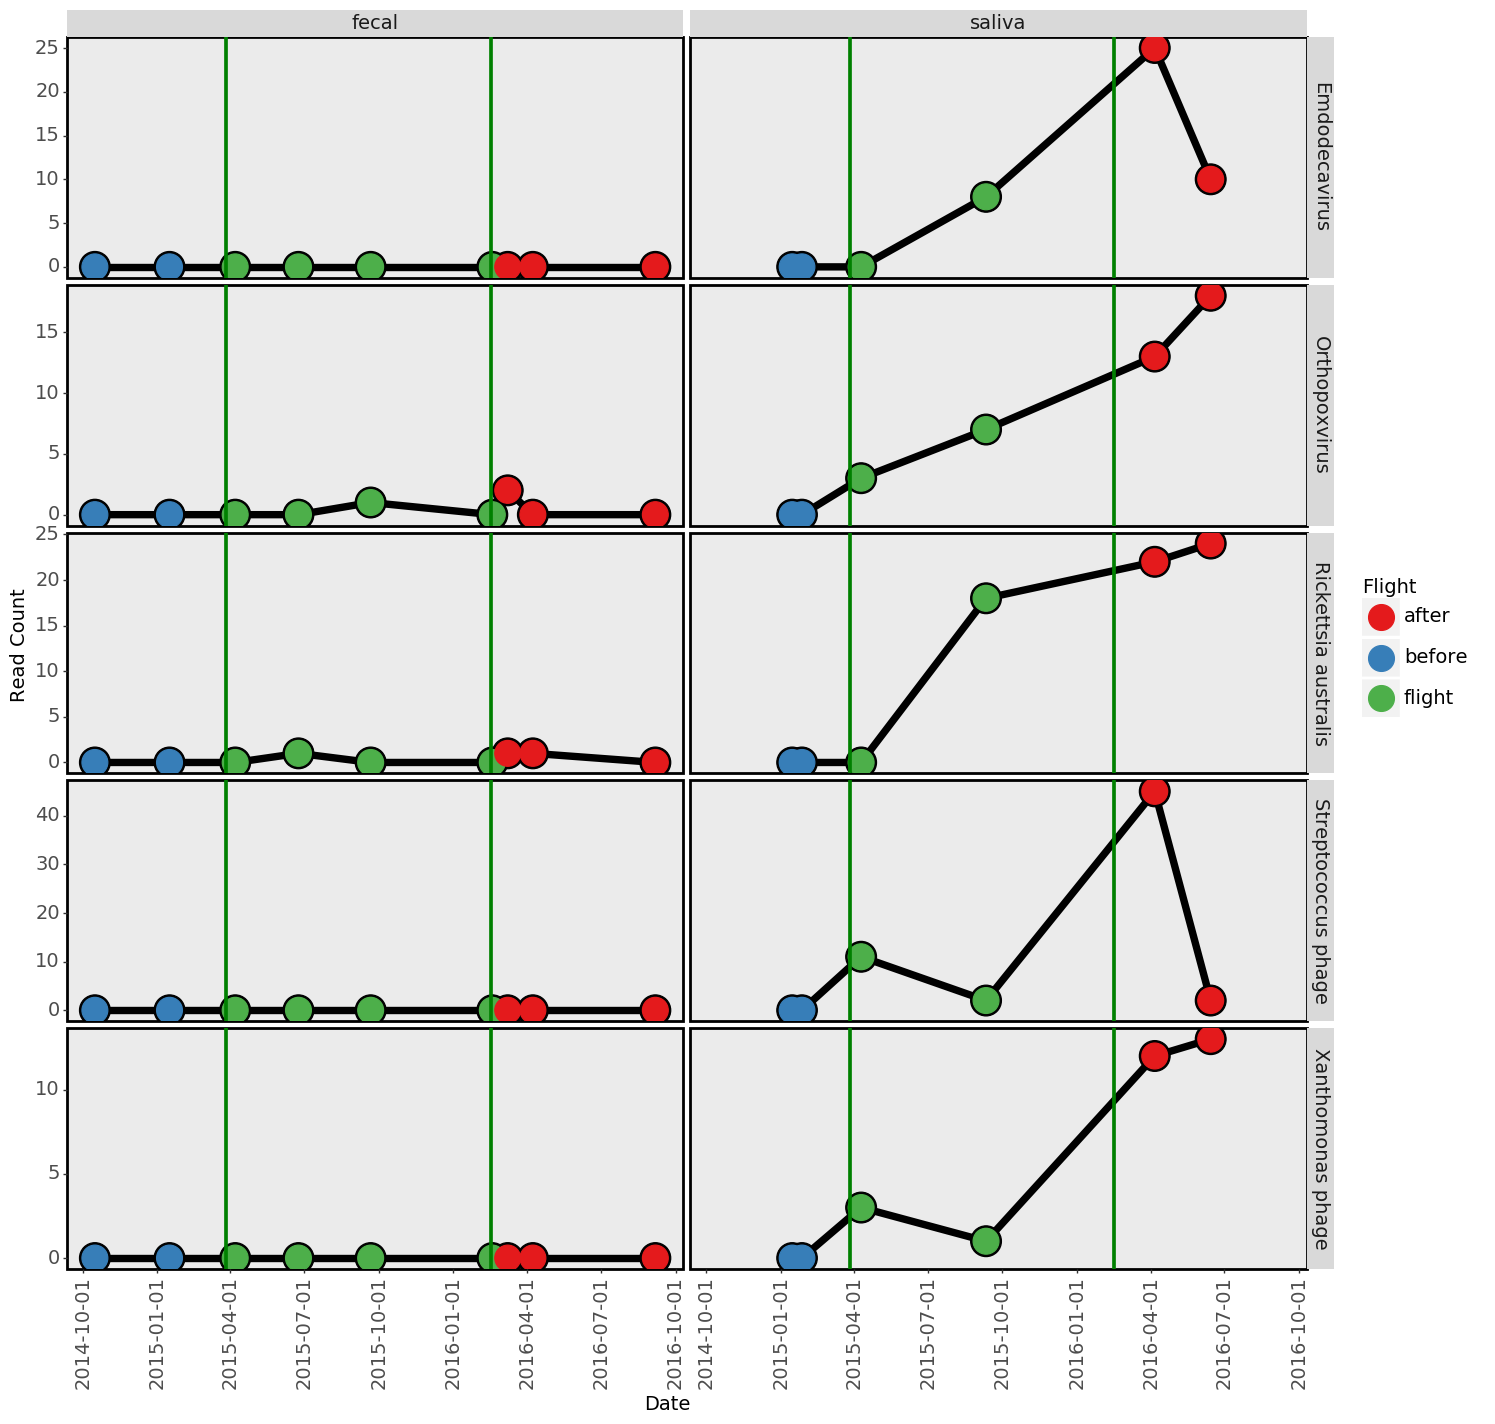
\includegraphics[width=0.99\textwidth]{figs/tw_flight_taxa.png}
%	\vspace{-20pt}
	\caption{\small{
	    Total number of reads observed in TW for different taxa not observed before flight. Green vertical bars indicate the start and end of flight. The \textit{Streptococcus phage} referenced is \textit{phiARI0004}, \textit{Xanthomonas phage} is \textit{vB XveM DIBBI},
	}}
    \label{fig:flighttaxa}
  \end{center}
%  \vspace{-20pt}
 % \vspace{1pt}
\end{figure}



\paragraph{Novel taxa in TW match environmental and commensal microbiomes}

We first examined the proportion of taxa observed in a given sample that were not observed in a previous sample from the same donor. Any newly observed taxa in given sample (e.g. stool) was annotated relative its presence in samples from other body or environmental sites (e.g saliva). For fecal samples, we segmented the previously unobserved taxa from each sample into four groups: taxa observed in any saliva sample taken before the given fecal samples, taxa observed in ISS samples but not observed in saliva, taxa observed in both ISS and saliva samples, and taxa that were not observed in either the ISS or the saliva. The same process was repeated for saliva samples but swapping fecal and saliva in the hierarchy. As expected,the time series of samples taken from the flight subject (TW) and ground control subject (HR) showed that earlier samples exhibited a greater proportion of novel organisms \ref{fig:taxasource}. Figure \ref{fig:hrtaxasource}. 

Of note, each sample contains a number of unobserved taxa that matched taxa from saliva/feces or the ISS (even before flight), indicating these are common commensal species on Earth or possibly organisms absorbed in previous missions. Indeed both astronauts had previously been in the space station across multiple missions though with a 10-fold difference in duration (TW has logged 520 total days on the ISS vs. 54 days for HR). Interestingly, when we examined the the fraction of taxa that match ISS taxa in pre-flight samples from TW compared to other samples from HR, a higher average rate ( 56\% ) of ISS-matching taxa was observed in pre-flight samples for TW relative to (HR  51\%), although not significant (p-value = 0.21). The fraction of taxa that matched different environments are listed in Table \ref{tbl:sourcepercents}. For both saliva and fecal microbiomes the large majority of taxa at each time point had already been observed in a previous sample from that site.  

A small number of taxa were never observed in any pre-flight sample from any body site but were observed in peri- and post-flight samples. We filtered for taxa that had no reads observed in pre-flight samples and had at least ten reads in at least two peri- or post-flight samples. These taxa were further filtered for taxa that were observed in at least two ISS samples. The resulting list included five taxa: two viral genera, two viral species (both phage), and one bacterial species: \textit{Rickettsia australis} (Figure \ref{fig:flighttaxa}). Given the generally low abundance of these taxa we cannot definitively rule out that they were present at an undetectable low threshold pre-flight. For comparison only 2 taxa (both viruses) met the above requirements but were not identified in ISS samples.
 
\begin{table}[]
\centering
\caption{This table gives the average overlap between emergent taxa in fecal and saliva microbiomes and microbiomes in other sites.}
\label{tbl:sourcepercents}
\begin{tabular}{lrr}
\toprule
Commensal Type &      Fecal &     Saliva \\
\midrule
Sites Where Taxa Originated     &            &            \\
%\midrule
Fecal Only       &  n/a &   8.7  \\
Saliva Only      &  10.2 &  n/a  \\
ISS Only        &  24.5 &  17.6 \\
Both ISS \& Saliva/Fecal        &  29.9 &  44.6 \\
Taxa not identified in another site &  35.5 &  29.1 \\
\bottomrule
\end{tabular}
\end{table}

\paragraph{Emergence of novel taxa in gut microbiomes exceeds repeated sampling} 

\begin{figure}
  \begin{center}
    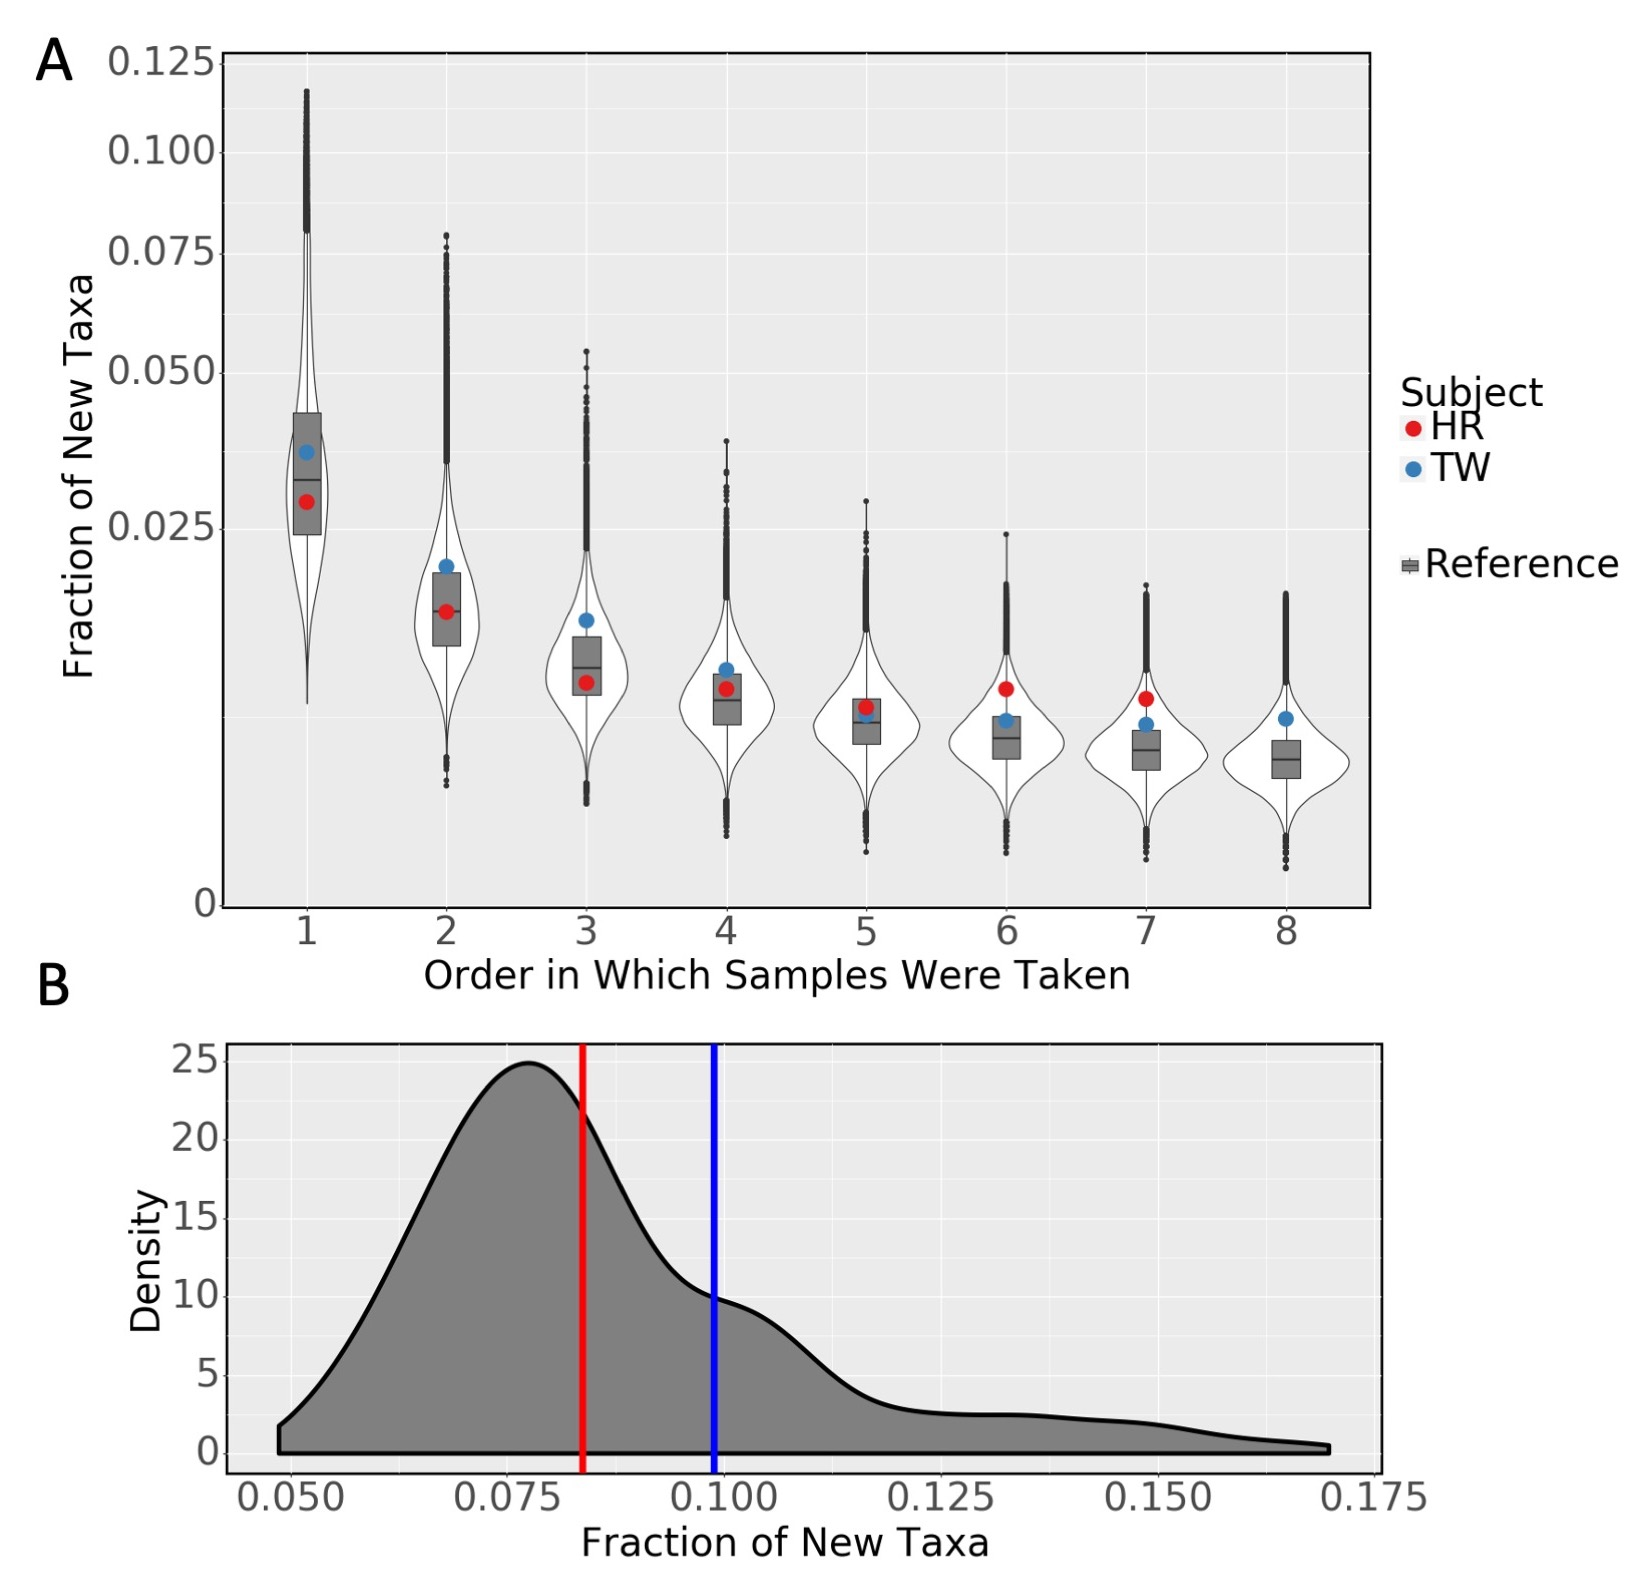
\includegraphics[width=0.99\textwidth]{figs/taxa_repeated_sampling.jpg}
%	\vspace{-20pt}
	\caption{\small{
	    A) The number of new taxa observed in TW and HR are higher than repeated resampling of the same fecal sample. The y-axis gives the number of new taxa at each time point (not observed at any previous time point) divided by the number of taxa in the first sample. The first time point is omitted from the plot because it is always 1 by construction. The x-axis gives the order of each sample (arbitrary for random subsample). Boxplots show the distribution of random subsamples. Colored points are the actual time series.
	    B) The number of unique taxa observed after the first time point divided by the number of taxa at the first time point. Same legend as (A)
	}}
    \label{fig:taxarepeated}
  \end{center}
%  \vspace{-20pt}
 % \vspace{1pt}
\end{figure}

To place these taxonomic trends in context, we investigated whether the sampling time series from TW and HR would identify more new taxa than repeated assays on an unchanging fecal sample. We compared the fecal microbiome time series of TW and HR to 243 repeated samples taken from a single fecal sample \citep{Sasada2020}, using 100,000 random sets of 9 samples (to match the twins' set size). The number of taxa in each sample that had not been observed in any previous sample were counted for each subset and normalized by the total number of taxa in the first sample. The time series for HR showed significantly more novel taxa than 99,971 (p 2.9e-4) random stool subsets, and TW had even more novel taxa than 99,990 (p 1e-4) random subsets (Figure \ref{fig:taxarepeated}). These results shows that the time series for TW and HR both consistently had more taxa than would be expected from resampling an unchanged fecal sample. 

\paragraph{Evidence of higher transfer rates on board the ISS}

We next calculated taxonomic diversity using Shannon's entropy for species profiles of each sample (Figure \ref{fig:taxadiv}). For both fecal and saliva samples from TW, the highest diversity was observed during flight, and this trend was not observed for HR in the same time intervals. We identified a significant increase in the number of previously unobserved taxa for samples taken from TW during flight (Figure \ref{fig:taxaflux}) compared to random permutations. 

To further characterize the significance of such transfer relative to the sampling set and the source, we performed a series of permutation tests. We first established the number of previously unobserved species found at each time point in the actual data from TW. We then randomly shuffled and relabeled these samples and counted species again for a total of 10,000 random permutations. We then counted the number of permutations where the number of species observed 'during flight' in the shuffled data was higher than the real data . For the fecal microbiome the actual number of observed taxa was higher than the shuffled data in 96.7\% of cases, for saliva 98.2\% of cases and for buccal the observed was higher than all other permutations. Repeating the same procedure on data from HR ('flight' status was arbitrarily assigned to the second, third, and fourth samples)  we observed 45.9\% for feces 98.2\% for saliva, and 80.1\% for buccal (more buccal samples were available for HR). Results were similar when the above procedure was repeated only with taxa found in ISS environmental samples.

\subsection{Strain level variation confirms microbial transfer}

\begin{table}[]
\centering
\caption{Size of regions that may have been transferred in kilobases. Gut-Saliva transfer means that a region was found in either the gut or saliva microbiome pre-flight, then found in the other during-flight. Environment transfer means a region was not found in either fecal or saliva microbiomes from TW pre-flight but was found during flight and was also present in the ISS.}
\label{tbl:covcounts}
\begin{tabular}{lrrr}
\toprule
{} &  Pre-flight &  Gut-Saliva transfer &  Environment transfer \\
\midrule
Bifidobacterium pseudocatenulatum &                  243.9 &                 92.4 &                  85.2 \\
Brevibacterium siliguriense       &                   18.7 &                  2.6 &                   3.1 \\
Gordonibacter urolithinfaciens    &                   37.8 &                 12.9 &                  21.2 \\
Bacillus albus                    &                   87.6 &                  7.0 &                  14.1 \\
Gluconobacter albidus             &                   10.2 &                  2.5 &                   1.3 \\
Fusobacterium necrophorum         &                   86.4 &                 18.0 &                  56.8 \\
Geobacillus stearothermophilus    &                   73.5 &                 13.7 &                  13.8 \\
Bifidobacterium catenulatum       &                  258.8 &                 17.5 &                  40.3 \\
Streptococcus viridans            &                 2319.6 &                 92.9 &                 221.8 \\
Vibrio alginolyticus              &                  211.0 &                 10.6 &                  89.7 \\
Staphylococcus sciuri             &                  179.0 &                 19.4 &                  37.4 \\
Pectobacterium parmentieri        &                  269.0 &                 22.7 &                  56.7 \\
Campylobacter lari                &                   42.0 &                  8.7 &                  18.1 \\
Atlantibacter hermannii           &                   66.4 &                 15.7 &                  30.6 \\
Bacillus tequilensis              &                   57.4 &                  6.0 &                   8.7 \\
Achromobacter ruhlandii           &                   49.8 &                 13.6 &                  11.7 \\
Serratia proteamaculans           &                   70.0 &                 11.2 &                   6.7 \\
Leptotrichia hongkongensis        &                  115.2 &                  0.7 &                  21.5 \\
Exiguobacterium antarcticum       &                   21.5 &                  4.4 &                   6.2 \\
Anoxybacillus amylolyticus        &                   11.5 &                  2.2 &                   2.3 \\
Kosakonia sacchari                &                   65.4 &                 16.0 &                  30.8 \\
Yersinia canariae                 &                   18.2 &                  8.2 &                   7.7 \\
Providencia heimbachae            &                   76.0 &                 12.1 &                   6.5 \\
Spirochaeta perfilievii           &                    2.7 &                  0.4 &                   0.7 \\
Cronobacter condimenti            &                   15.2 &                  8.5 &                  18.8 \\
Brenneria rubrifaciens            &                   13.2 &                  5.7 &                   7.3 \\
Staphylococcus simiae             &                   20.8 &                  1.5 &                   6.2 \\
\bottomrule
\end{tabular}
\end{table}

\paragraph{Novel genome regions in flight found in environmental and commensal microbiomes}

Given the higher overall transfer rate of species on the ISS, we next examined the strain emergence and persistence (post-flight) of such species. For all species showing significantly greater abundance during and after flight in TW than before flight,  reads were mapped to known reference strains from these taxa. We looked at the coverage of reference genomes at each stage of flight (concatenating samples from the same stage) and in the ISS and grouped regions into three categories: regions which were covered before flight, regions that were covered before flight in either gut or saliva samples but not observed in the other until flight, and regions that were not observed in either gut or saliva samples until flight but were found in the environment. \textit{Fusobacterium necrophorum}  and \textit{Serratia proteamaculans} Figure \ref{fig:fnecro} and Figure \ref{fig:sprota}. The total size of these genomic regions for all tested taxa are listed in  Table \ref{tbl:covcounts}.

For the selected taxa, the average environmental transfer of genomic regions were 32.2\% of the size of pre-flight regions, whereas gut-saliva transfers were lower at 19.9\%. The taxa with the (proportionally) largest transferred regions \textit{Cronobacter condimenti}, had 55.9\% gut-saliva transfer and 123.7\% environmental transfer. The presence of (in some taxa) large genomic regions that were not covered until flight strongly suggests that individual species are undergoing flux with new strains and genes migrating into commensal microbiomes. 

\paragraph{Microbial SNPs match environmental and commensal microbiomes}



\begin{figure}
  \begin{center}
    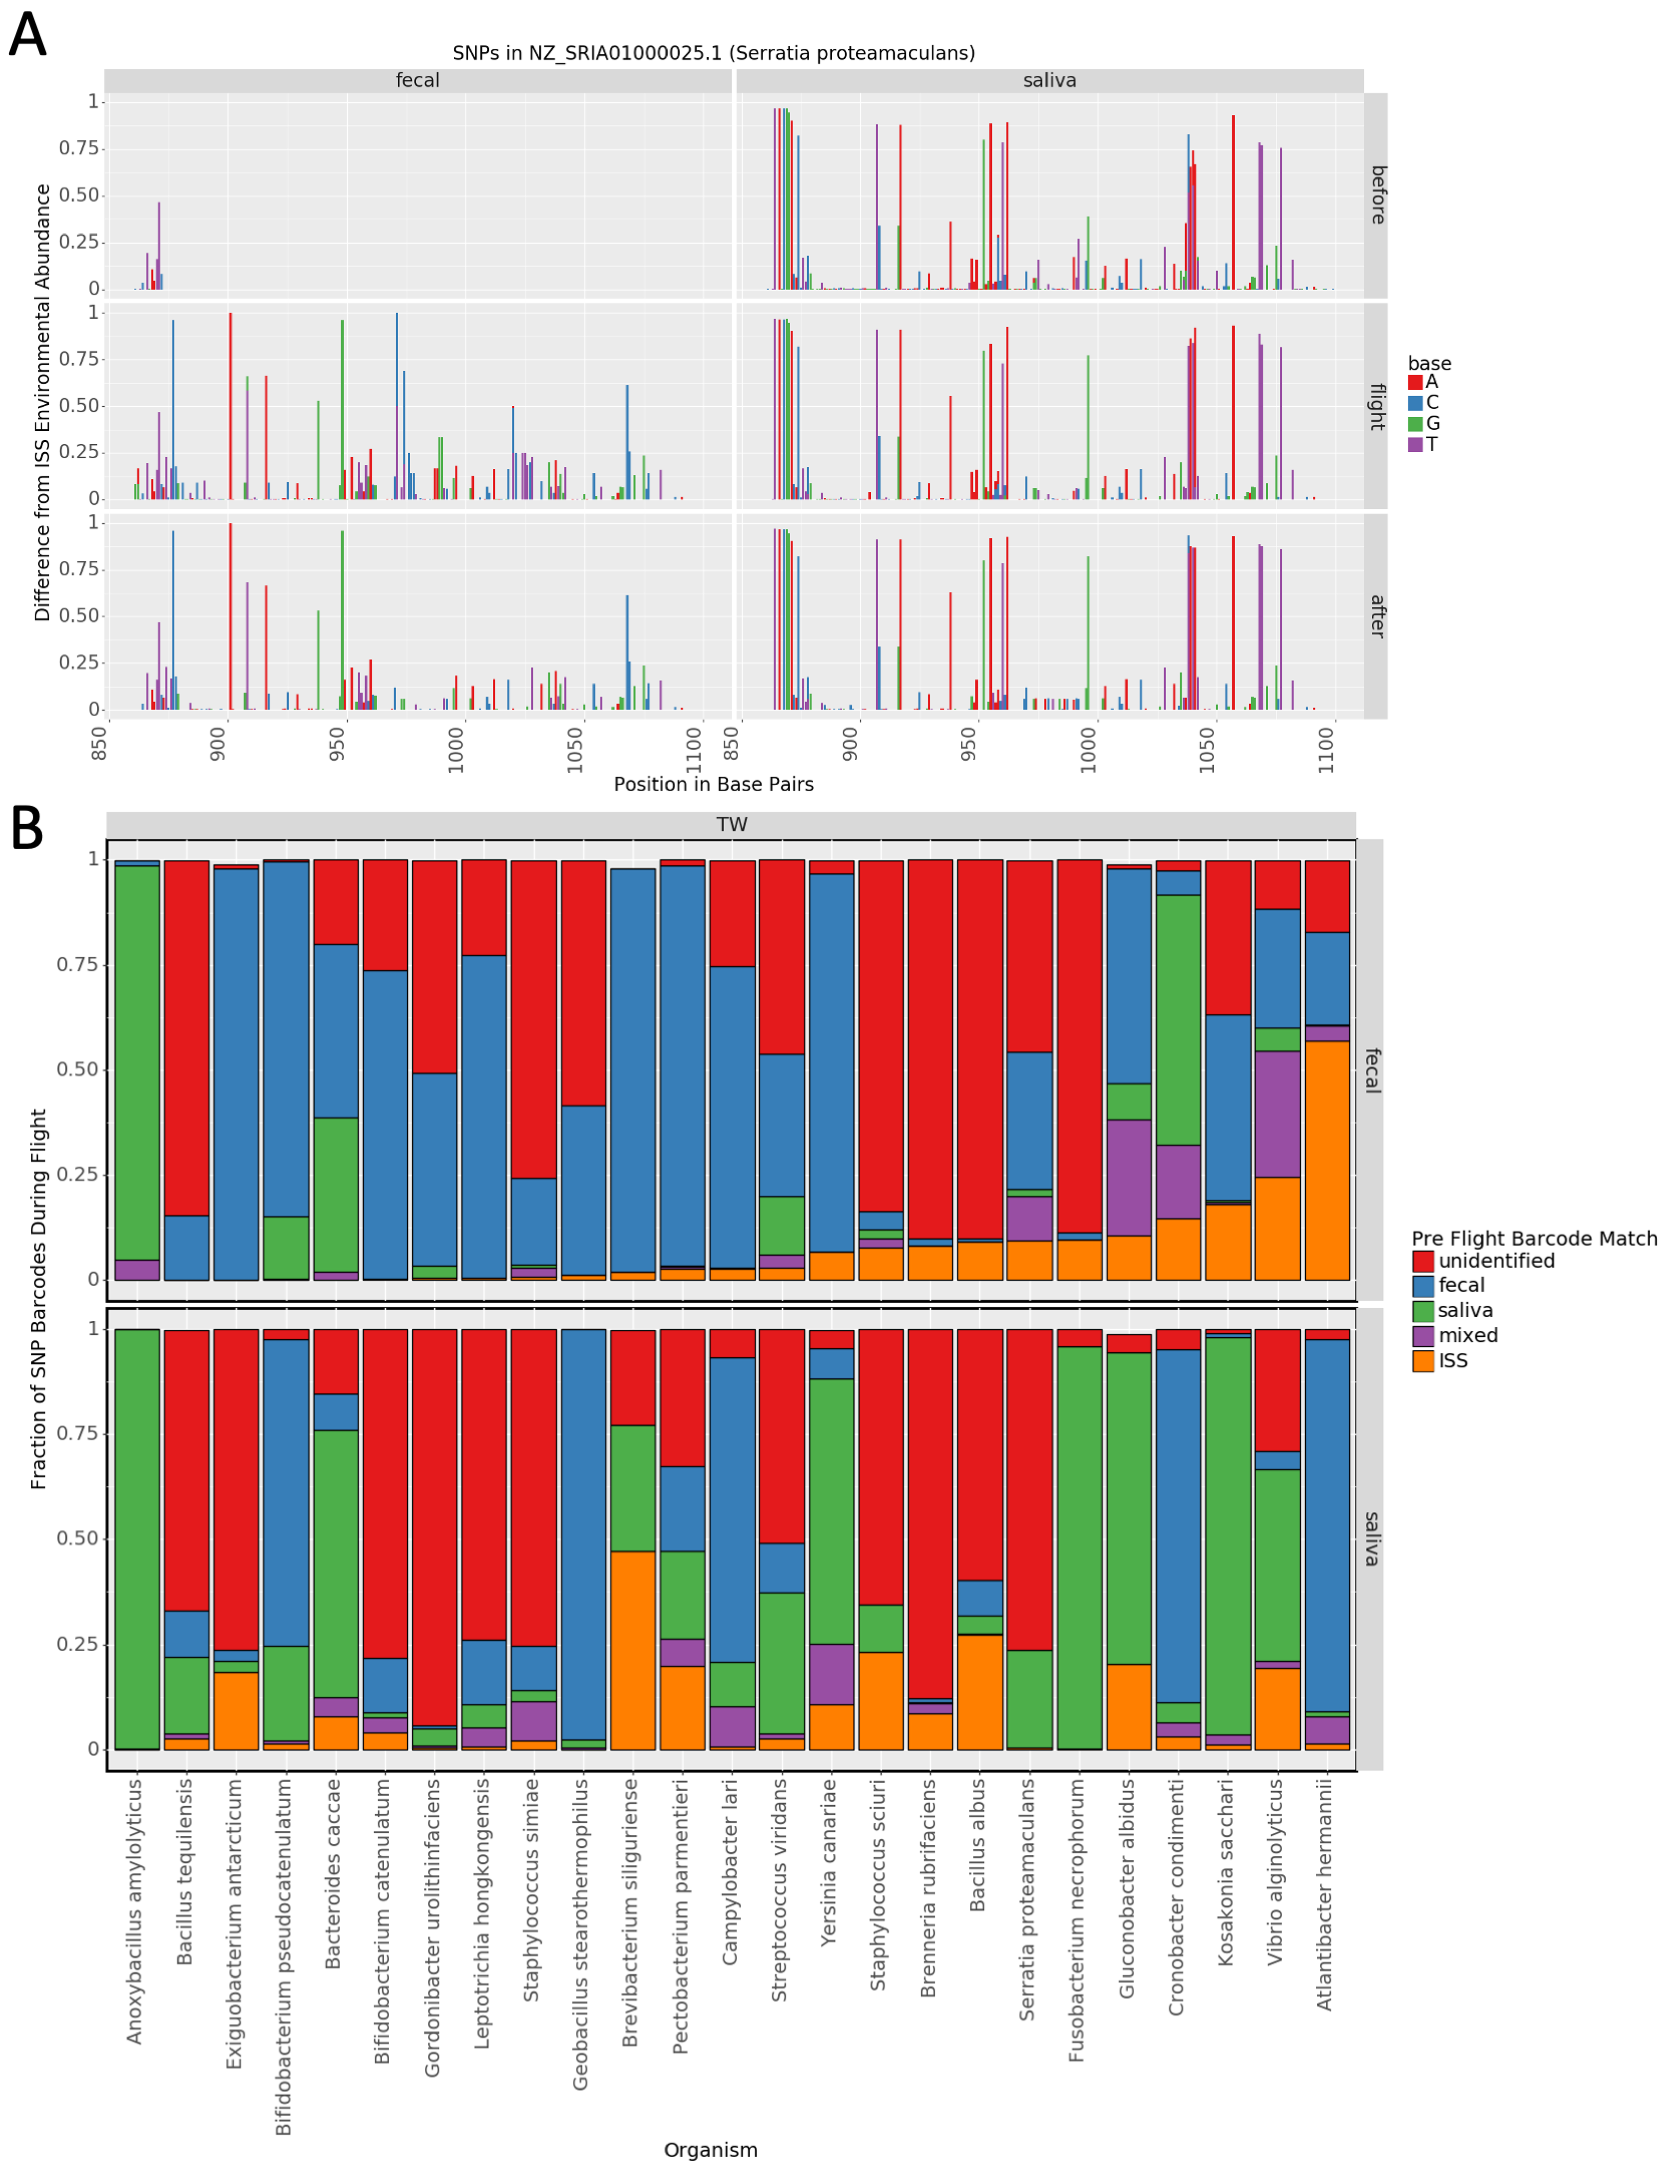
\includegraphics[width=0.99\textwidth]{figs/snp_bcs.png}
%	\vspace{-20pt}
	\caption{\small{
	    A) An example set of SNPs found in Serratia proteamaculans. The abundance of each SNP is shown relative to the frequency of the base found in the ISS at each position. A tall column indicates a base was low abundance in the ISS environment. In this case the SNPs shown for the fecal (left) strain match a secondary strain in the environment and constitute a candidate for transfer from the environment to the gut microbiome.
	    B) Pre-flight sources of different SNP barcodes observed in TW during flight. Each SNP barcode in peri-flight samples from TW was matched to barcodes in pre-flight samples from TW and ISS samples. The fraction of barcodes matching each source is shown. For fecal samples barcodes labeled as saliva did not match fecal samples and vice versa. Barcodes labeled as matching ISS were not found in either fecal or saliva samples.
	}}
    \label{fig:bcsources}
  \end{center}
%  \vspace{-20pt}
 % \vspace{1pt}
\end{figure}


Once the candidate genomic regions were identified, we next mapped co-occurring clusters of SNPs (haplotypes) in the selected taxa listed above in all samples from TW, HR, and the ISS (Figure \ref{fig:bcsources}. We matched microbial haplotypes from TW during flight to possible sources in pre-flight TW samples and ISS samples. Pre-flight fecal samples we considered four groups: haplotypes found in pre-flight fecal samples, haplotypes found in pre-flight saliva but not fecal samples, haplotypes found in the ISS but neither saliva nor fecal, and haplotypes not observed in any other group. 

The pre-flight sources of haplotypes varied by the species being investigated (Figure \ref{fig:bcsources}B). Some species, such as \textit{Cronobacter condimenti} showed an apparent flip of strains from the gut microbiome to saliva and vice versa. Other taxa, like \textit{Atlantibacter hermannii}, showed a large fraction of haplotypes that matched environmental haplotypes in the gut microbiome. Some taxa, like \textit{Bifidocaterium catenulatum} showed little similarity to any potential external source.



\subsection{Transfer Case Study: Serratia Proteamaculans}

\paragraph{SP is a candidate persistent transfer}

\begin{figure}
  \begin{center}
    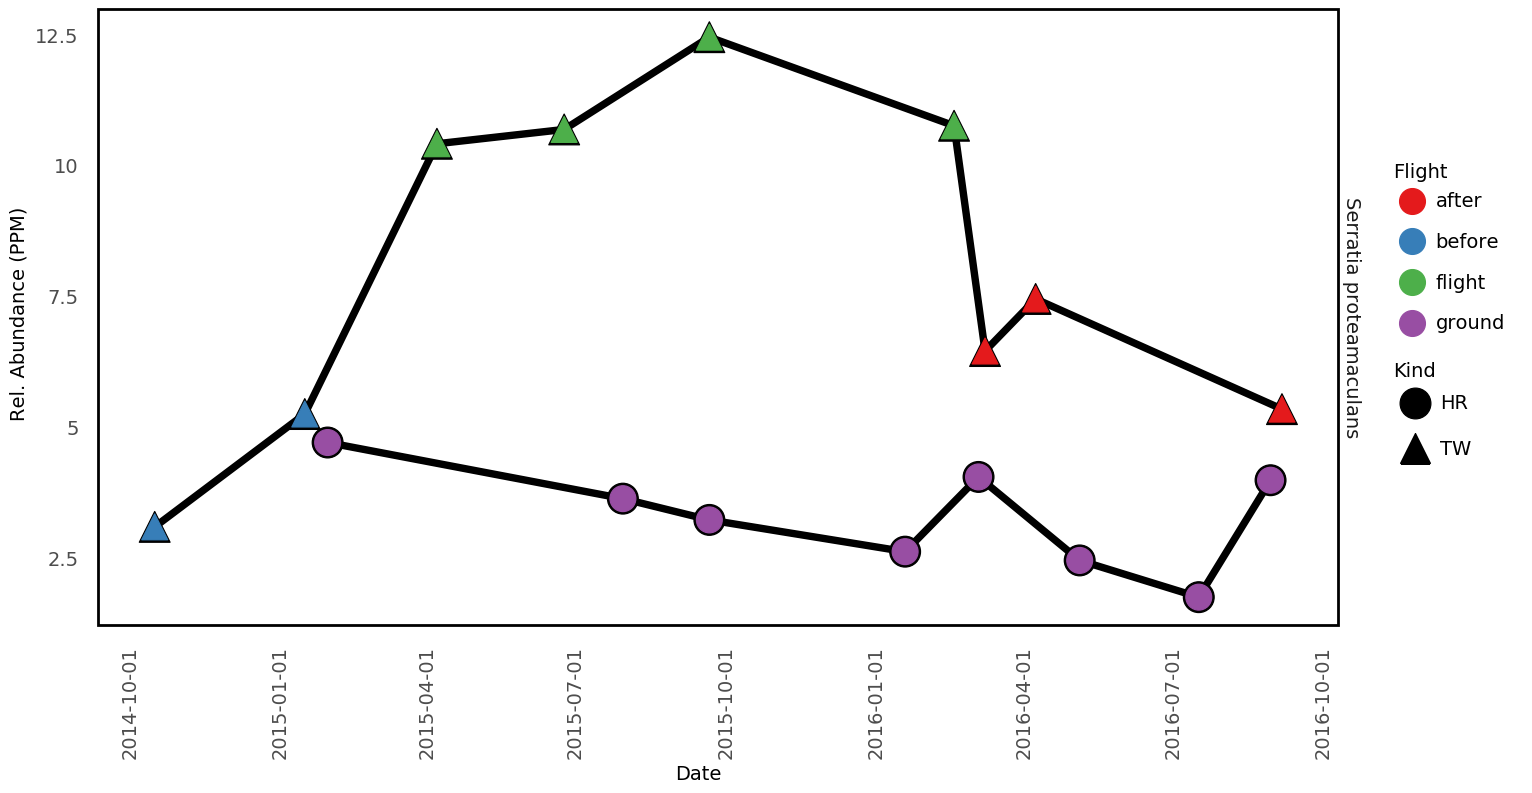
\includegraphics[width=0.99\textwidth]{figs/sp_abundance.png}
%	\vspace{-20pt}
	\caption{\small{
	    Relative abundance of \textit{Serratia proteamaculans} in fecal samples from TW and HR. Relative abundance is given in units of parts per million.
	}}
    \label{fig:abundance}
  \end{center}
%  \vspace{-20pt}
 % \vspace{1pt}
\end{figure}

We identified SP as a candidate persistent transfer, a species that was found in ISS environmental samples and was significantly more abundant in peri and post flight fecal samples from TW than other fecal samples. As a whole SP was only found at low levels in fecal samples in TW pre-flight, was significantly more abundant during flight, and dropped to an intermediate level after flight (Figure \ref{fig:abundance}). No major variation in abundance was observed for the control twin HR. SP was roughly uniformly abundant in the saliva before during and after flight.

\paragraph{Regions of the SP genome are found in TW fecal samples only after arrival at the ISS}

\begin{figure}
  \begin{center}
    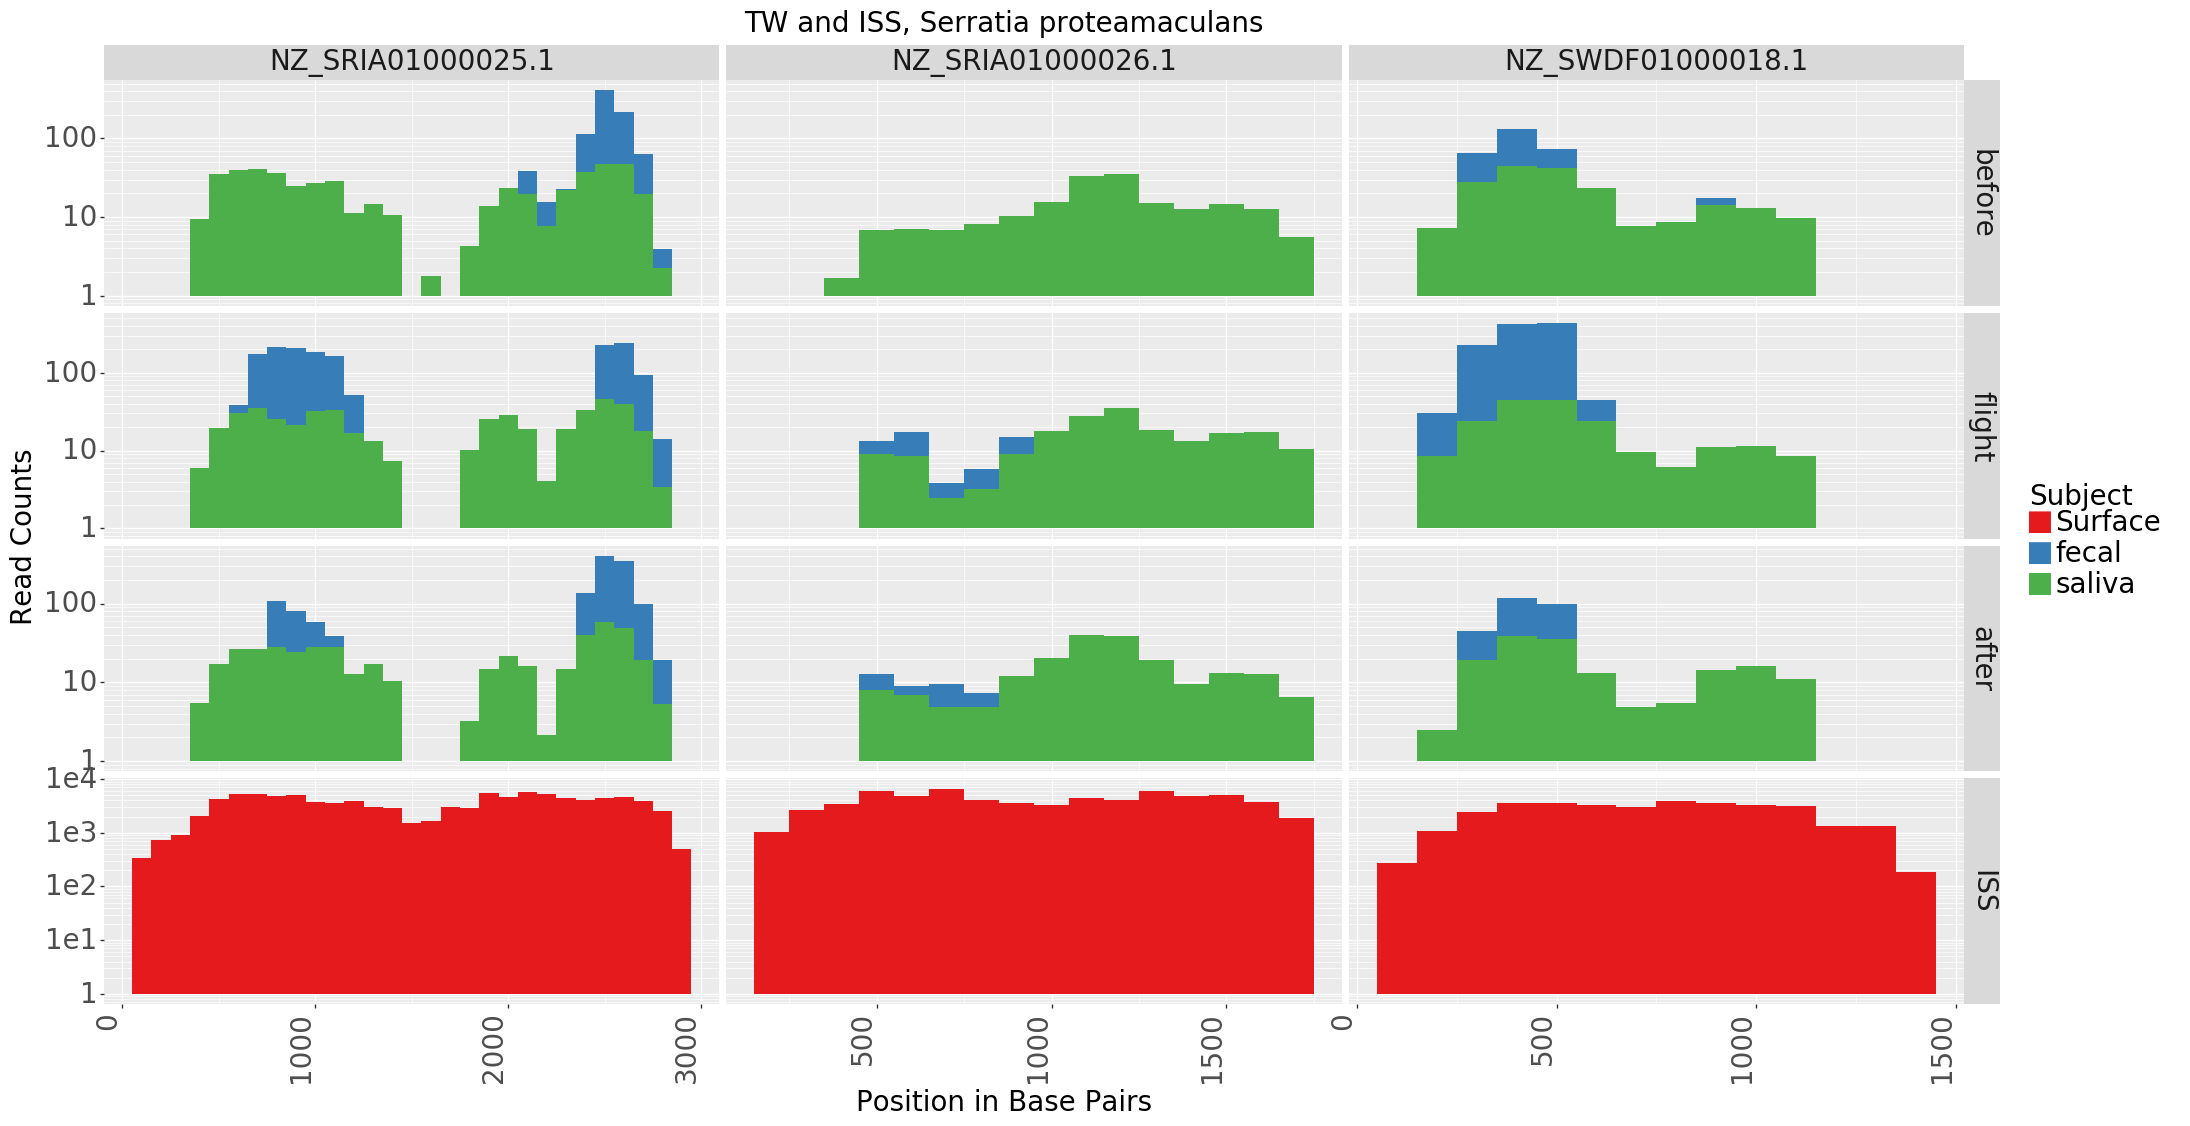
\includegraphics[width=0.99\textwidth]{figs/sprota_read_recruit.png}
%	\vspace{-20pt}
	\caption{\small{
	    Coverage of candidate persistent transfer regions of the \textit{Serratia proteamaculans} genome.
	}}
    \label{fig:sprota}
  \end{center}
%  \vspace{-20pt}
 % \vspace{1pt}
\end{figure}

We identified regions of the SP genome which appeared in fecal samples after TW was on board the ISS. We found three such regions totaling about 1.5kbp. The abundance of these regions roughly matched the overall pattern seen for SP. Very low or undetectable pre-flight, a high during flight, and an intermediate level post flight (Figure \ref{fig:sprota}). These regions were all well covered from ISS environmental samples.

Total coverage of the SP genome in TW from all available samples 29.2kbp. Before flight 8.9kbp was covered, during 17.2kbp and after 19.0kbp. However some of these regions were either quite small or not covered in both peri and post flight. As such 1.5kbp represents a reasonable fraction of the amount of SP genome covered in TW but should only be interpreted as evidence for the transfer of particular genes. 


\subsection{SNPs in post-arrival regions match a secondary environmental strain}

We analyzed one of the above regions (of about 250bp) for SNPs (Figure \ref{fig:bcsources}A) and identified SNPs in samples from TW which were either not found in the ISS environment or were found at different proportions. We identified 9 SNPs in this region during flight that were found in fewer than half of the ISS environmental samples. Of these 9 SNPs 6 were found after the conclusion of flight. We note that all of these 9 SNPs were found in ISS environmental samples at some proportion.

Next we used the SNP clustering technique described in the methods to determine if the 9 peri-flight SNPs we identified could come from the same strain. We identified corresponding groups of 8 SNPs in TW and 9 SNPs in the ISS environment. The 8 SNP group in TW included 8 out of the 9 peri-flight SNPs. The 9 SNP group from the ISS environment included these 8 SNPs as well as one SNP not identified in TW. This leads us to the conclusion that the strain found in TW likely represented a secondary strain in the ISS environment. 

